\documentclass{scrartcl}

\usepackage[utf8]{inputenc}
\usepackage[T1]{fontenc}
\usepackage{lmodern}
\usepackage[english]{babel}
\usepackage{hyperref}
\usepackage{graphicx}
\usepackage{booktabs}
\usepackage{wrapfig}
\usepackage{listings}
\usepackage{xcolor}

\clubpenalty = 10000 
\widowpenalty = 10000 
\displaywidowpenalty = 10000

\colorlet{punct}{red!60!black}
\definecolor{background}{HTML}{EEEEEE}
\definecolor{delim}{RGB}{20,105,176}
\colorlet{numb}{magenta!60!black}

\lstdefinelanguage{json}{
    basicstyle=\normalfont\ttfamily\scriptsize,
    showstringspaces=false,
    breaklines=true,
    frame=lines,
    backgroundcolor=\color{background},
    literate=
     *{0}{{{\color{numb}0}}}{1}
      {1}{{{\color{numb}1}}}{1}
      {2}{{{\color{numb}2}}}{1}
      {3}{{{\color{numb}3}}}{1}
      {4}{{{\color{numb}4}}}{1}
      {5}{{{\color{numb}5}}}{1}
      {6}{{{\color{numb}6}}}{1}
      {7}{{{\color{numb}7}}}{1}
      {8}{{{\color{numb}8}}}{1}
      {9}{{{\color{numb}9}}}{1}
      {:}{{{\color{punct}{:}}}}{1}
      {,}{{{\color{punct}{,}}}}{1}
      {\{}{{{\color{delim}{\{}}}}{1}
      {\}}{{{\color{delim}{\}}}}}{1}
      {[}{{{\color{delim}{[}}}}{1}
      {]}{{{\color{delim}{]}}}}{1},
}

\titlehead{University of Koblenz-Landau}
\title{WikiTax - A tool for taxonomy extraction based on the Wikipedia Category Graph}
\author{Dominik Mosen (dmosen@uni-koblenz.de)}

\begin{document}
\maketitle

% \begin{abstract}
% Lorem ipsum dolor sit amet, consetetur sadipscing elitr, sed diam nonumy eirmod tempor invidunt ut labore et dolore magna aliquyam erat, sed diam voluptua. At vero eos et accusam et justo duo dolores et ea rebum. Stet clita kasd gubergren, no sea takimata sanctus est Lorem ipsum dolor sit amet. Lorem ipsum dolor sit amet, consetetur sadipscing elitr, sed diam nonumy eirmod tempor invidunt ut labore et dolore magna aliquyam erat, sed diam voluptua. At vero eos et accusam et justo duo dolores et ea rebum. Stet clita kasd gubergren, no sea takimata sanctus est Lorem ipsum dolor sit amet.
% \end{abstract}

\section{Introduction}
Wikipedia - as a collaboratively created encyclopedia - uses several means to organise its information. Examples include links from articles to other related articles forming an article graph \cite{ZeschGurevych2007analysis}, stand-alone lists\footnote{\url{http://en.wikipedia.org/wiki/Wikipedia:Manual_of_Style/Stand-alone_lists}, last visit 17th April 2013} listing articles that describe a certain theme, or portals\footnote{\url{http://en.wikipedia.org/wiki/Wikipedia:Portal}, last visit 17th April 2013} which are meant to introduce users to the main topics of Wikipedia. Besides these methods, categories\footnote{\url{http://en.wikipedia.org/wiki/Wikipedia:FAQ/Categories}, last visit 17th April 2013} can be used to classify articles. Therefore, categories are defined that again contain other categories and articles thus shaping a category graph \cite{ZeschGurevych2007analysis}. 

While the main purpose of the mentioned means is to provide users with additional or related information to certain topics, the given data can also be used to derive domain specific taxonomies which can be leveraged in several areas, such as in the 101companies project \cite{FavreLaemmel101}. This project provides knowledge concerning software technologies, software languages and technological spaces. As it is wiki-based and has similar requirements for structuring its information as Wikipedia, it should be examined how Wikipedia handles the problem of organising its content. In this context, Wikipedia's knowledge on computer science topics could be helpful to improve the 101companies' wiki\footnote{\url{http://101companies.org/}, last visit 17th April 2013}. At the present time, efforts are made to incorporate the Semantic MediaWiki extension\footnote{\url{http://semantic-mediawiki.org/}, last visit 17th April 2013} into the 101companies' wiki, which makes MediaWiki\footnote{\url{http://www.mediawiki.org/wiki/MediaWiki}, last visit 17th April 2013} contents computer-processable by adding semantic annotations. To develop a meaningful structure, condensed information from Wikipedia on relevant topics could serve as a starting point or reveal missing or under-represented subjects.

Therefore, this paper describes the tool \emph{WikiTax}, which supports the creation of taxonomies based on the Wikipedia category graph and helps to analyse the structure of Wikipedia for desired domains. For this purpose, the structure the Wikipedia Category Graph is described in §\ref{sec:category_graph}, before §\ref{sec:wiki_tax} explains the developed tool and gives operating instructions. §\ref{sec:conclusion} summarises this paper and gives a short outlook.

\section{The Wikipedia Category Graph}
\label{sec:category_graph}
Categories in Wikipedia are hierarchically ordered. More precisely, the hierarchy of categories can be considered as a graph consisting of vertices representing the categories and of directed edges indicating a subcategory relationship. Although Wikipedia does not enforce the hierarchical ordering of categories, this holds true for most of them. According to \cite{ZeschGurevych2007analysis}, the category graph of the German Wikipedia from May 15, 2006 had 7 backlinks causing cycles (i.e. links pointing from a hierarchically lower category to a higher one and thus invalidating the hierarchical order). Although not explicitly mentioned, the dump reports on Wikipedia\footnote{\url{http://en.wikipedia.org/wiki/Wikipedia:Dump_reports}, last visit 17th April 2013} indicate that cycles are not by intention. Ignoring these rare backlinks, the category graph can be transformed into a directed acyclic graph (DAG), which enables a hierarchical representation.

\section{WikiTax}
\label{sec:wiki_tax}
\textit{WikiTax} utilises the existing Wikipedia category graph to derive taxonomies. The following sections describe the basic data model of \emph{WikiTax} and explain the general workflow when using it. As the main idea of this workflow is to reduce the Wikipedia category graph until a meaningful structure remains, there are several mechanisms to support this reduction process, which is discussed in section \ref{sec:support}. Section \ref{sec:review} treats the possibilities of reviewing and reverting decisions during the reduction, while the last section \ref{sec:save} deals with saving, loading and exporting results and the data formats provided for this purpose.

\subsection{The data model}

\begin{figure}[htb]
\centering
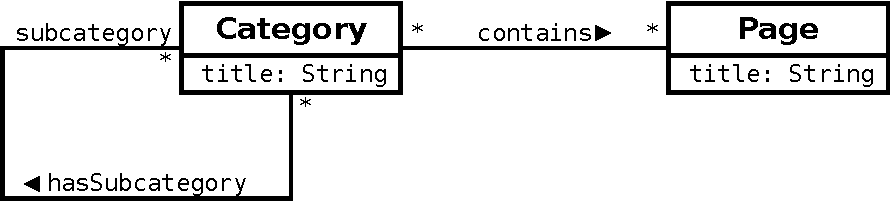
\includegraphics[width=0.6\textwidth]{figures/simple_schema.pdf} 
\caption{Schema of the Wikipedia category graph}
\label{fig:simple_schema}
\end{figure}

As mentioned before, \emph{WikiTax} works with the Wikipedia category graph. Figure \ref{fig:simple_schema} depicts the data model which serves as a basis for \emph{WikiTax}. It consists of \texttt{Category}s and \texttt{Page}s which are connected by \texttt{hasSubcategory}- or \texttt{contains}-associations. \texttt{Category}s correspond to Wikipedia categories and \texttt{Page}s to Wikipedia articles. The \texttt{hasSubcategory}-association indicates a subcategory relationship between two Wikipedia categories whereas the \texttt{contains}-association describes that a Wikipedia article is contained in a Wikipedia category.

\subsection{The Workflow}
The derivation of a taxonomy using \emph{WikiTax} is essentially done in two steps. At first, a category subgraph - starting at a given root category - is extracted from Wikipedia. Afterwards, this graph is incrementally reduced until a meaningful structure remains. The user is guided through these steps by two separated views that will be discussed in the following sections.

\subsubsection{Extracting the category subgraph}

\begin{figure}[ht]
  \centering
  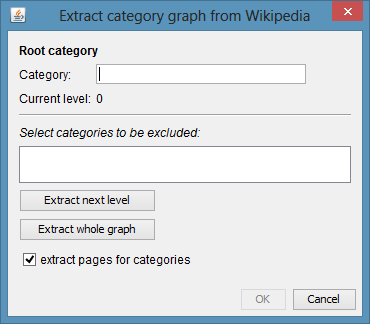
\includegraphics[scale=0.60]{figures/extraction_dialog.png}
  \caption{The extraction dialog}
  \label{fig:extaction_dialog}
\end{figure}

To extract a category subgraph, the extraction dialog pictured in Figure \ref{fig:extaction_dialog} is opened by selecting \texttt{File > Extract} from the menu bar after \emph{WikiTax} was started. The user only needs to enter a valid Wikipedia category which is defined as the root category for the extraction process. After the \texttt{Extract whole graph} or \texttt{Extract next level} button has been clicked, the extraction starts. In both cases, the Wikipedia category graph is traversed in breadth-first search order. This is done by following all \texttt{containsPage}- and \texttt{hasSubcategory}-edges, starting at the given root category. The traversal is executed by running successive queries against Wikipedia via the MediaWiki API\footnote{\url{http://en.wikipedia.org/w/api.php}, last visit 17th April 2013}.

In the first case, the complete subgraph is traversed and thereby extracted in one run whereas in the second case, only one level is processed at a time. The latter procedure permits to exclude individual categories from the extracted graph at a particular level and to continue the extraction for the next level. This is especially helpful if it is known that the category in question is unnecessary and relatively comprehensive, and would therefore consume a lot of time when extracting.\footnote{Be aware that - on extraction - the exclusion of categories is purely intended to reduce time effort and complexity of the extracted graph. If you are unsure about exclusion of categories, keep them as they can still be excluded in the reduction step (cf. section \ref{sec:reduce}).} 

No matter which extraction option was selected, the progress will be displayed in a progress dialog. The extraction can be cancelled at any time by clicking the \texttt{Cancel} button, but every progress since the last extraction step will be lost.

If a satisfying category subgraph was extracted, the extraction dialog is accepted by clicking the \texttt{OK} button. After an optional saving of the extracted graph, the `graph reduction step' begins.

\subsubsection{Reducing the graph}
\label{sec:reduce}

\begin{figure}[ht]
\centering
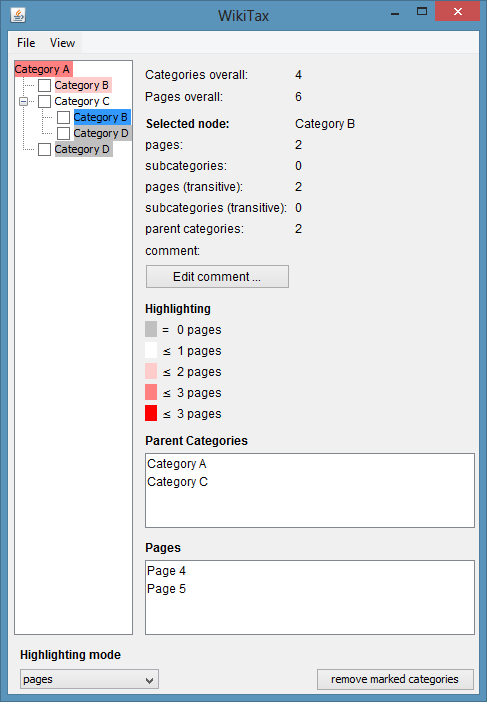
\includegraphics[scale=0.5]{figures/WikiTax_selected_node.png}
\caption{The reduction view}
\label{fig:reduction_view}
\end{figure}

Although dealing with a graph, the reduction view (figure \ref{fig:reduction_view}) shows it as a (hierarchical) tree structure. This tree is produced by traversing the graph in depth-first search order. Thereby, cycles are detected and the responsible edges (backward arcs) are blacklisted and ignored. This produces a directed acyclic graph (DAG). Every edge of this DAG corresponds to a tree node in the tree view displayed in the reduction view. As the root category does not have an incoming edge in the DAG (because it was the first category to be extracted), no correspondent edge can be given. Nevertheless the root category is still part of the category tree. The relationships between a category graph and its appropriate category tree can be seen in figure \ref{fig:graph_tree}.

\begin{figure}[ht]
\centering
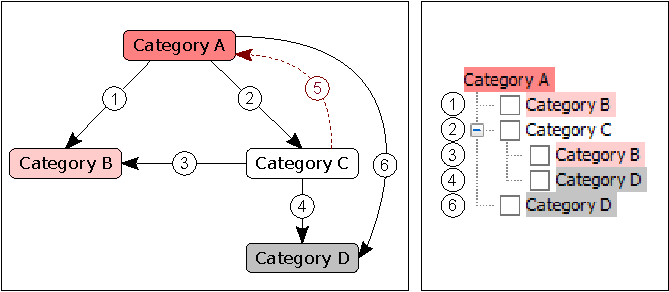
\includegraphics[scale=0.8]{figures/graph_tree.pdf}
\caption{Correspondence between a category graph and a category tree. As \texttt{Category A} is the root category it has no corresponding edge. Notice that edge number 5 has no corresponding tree node because it causes a cycle and is therefore not part of the DAG.}
\label{fig:graph_tree}
\end{figure}

The reduction is done by marking nodes through clicking check boxes in the reduction view and by removing them with the activation of the \texttt{remove blacklisted categories} button. Internally, the removal is done by blacklisting edges corresponding to the tree nodes in the underlying category graph. The influence of removing a tree node is depicted in figure \ref{fig:graph_tree_blacklisted}. Moreover, every tree node (except for the root node) can be provided with a comment that is meant to indicate the reason for the exclusion.

\begin{figure}[ht]
\centering
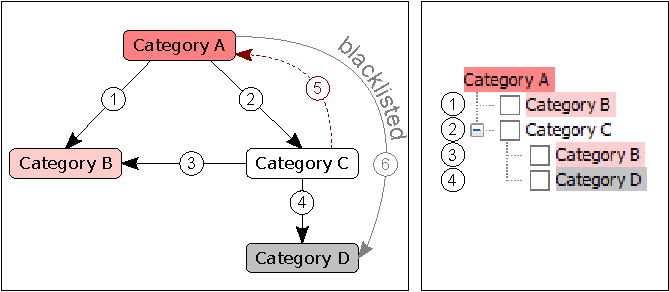
\includegraphics[scale=0.8]{figures/graph_tree_blacklisted.pdf}
\caption{Influence of a removal of a tree node to the graph}
\label{fig:graph_tree_blacklisted}
\end{figure}

After several iterations of removing tree nodes, a reasonable structure that resembles a domain specific taxonomy should evolve. If it does not, this could be due to a badly organised structure of Wikipedia or an inadequate reduction of categories by the user.  However, if an incomplete or unsatisfying structure is obtained, it may serve as a starting point for designing one.

\subsection{Reduction process support}
\label{sec:support}
The reduction process described in the preceding section is highly dependent on the user's knowledge which enables him or her to include or exclude categories. \emph{WikiTax} has different means to support users in this decision process: that is providing general data about the graph, data for the currently selected tree node and a highlighting system giving visual information which categories could be important or not.

\subsubsection{General data}

The general data (figure \ref{fig:general_data}) contain information that is not specific for a certain tree node but represent information concerning the whole underlying category graph (i.e. the data can be displayed even if no node is selected):

\begin{figure}[ht]
\centering

\includegraphics[scale=0.7]{figures/general_data.png}
\caption{General data}
\label{fig:general_data}
\end{figure}

\begin{description}
\small
\item[Categories overall] The number of different categories the category graph contains overall.
\item[Pages overall] The number of different pages the category graph contains overall.
\end{description}

Notice, even if the tree view has several occurrences of the same category or page - based on the graph -, they are only counted once.

\subsubsection{Data for a selected tree node}

As previously mentioned, every tree node refers to an edge pointing to a category in the category graph. When a tree node is selected, the following data regarding the targeted category are displayed (figure \ref{fig:node_data}):

\begin{figure}[h]
\centering
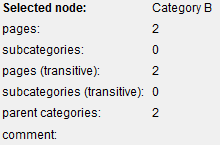
\includegraphics[scale=0.7]{figures/node_data.png}
\caption{Selected node data}
\label{fig:node_data}
\end{figure}

\begin{description}
\small
\item[pages] The number of pages directly contained in the selected category
\item[categories] The number of subcategories directly contained in the selected category
\item[pages (transitive)] The number of pages directly or indirectly contained in the selected category
\item[categories (transitive)] The number of subcategories directly or indirectly contained in the selected category
\item[parent categories] The number of categories this category is contained in
\end{description}

It holds especially for \texttt{pages (transitive)} and \texttt{categories (transitive)} that the calculation is based on the graph. Hence, they represent the number of different pages or categories that are reachable from the selected category in the category graph. This means that no category or page is counted twice.

\subsubsection{The highlighting system}

The highlighting modes listed below can be selected in the highlighting combo box at the lower left of the reduction view:

\begin{itemize}
	\item pages 
	\item categories
	\item pagesTransitive
	\item categoriesTransitive
\end{itemize}

\begin{figure}[ht]
\centering
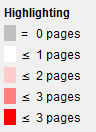
\includegraphics[scale=0.6]{figures/highlighting_pages.png}
\caption{Legend for the highlighting mode \texttt{pages}}
\label{fig:highlighting_pages}
\end{figure}

For the highlighting of the \texttt{pages} (figure \ref{fig:highlighting_pages}), thresholds are calculated to colour the tree nodes. Therefore, the first quartile, the median, the third quartile and the maximum are calculated based on the count of pages directly contained in a category while ignoring categories containing zero pages. Based on these thresholds, the classification shown in table \ref{tab:highlighting_pages} is applied to the tree nodes to determine their colourings. Therefore, the conditions are checked top-down. The first valid condition determines the colouring. The colouring of the \texttt{categories} mode is equally defined but instead of the contained pages count, the contained categories count is used.

\begin{table}[ht]
\scriptsize
\centering
\begin{tabular}{ll}
\toprule 
\textbf{Colouring} & \textbf{Condition} \\
\midrule
gray & pages = 0 \\ 
\midrule
white & pages $\le$ 1. quartile \\ 
\midrule
light red & pages $\le$ median \\ 
\midrule
medium red & pages $\le$ 3. quartile \\ 
\midrule
dark red & pages $\le$ maximum \\ 
\bottomrule
\end{tabular} 
\caption{Highlighting of tree nodes for mode \texttt{pages}}
\label{tab:highlighting_pages}
\end{table}

If highlighting was applied to transitive values, quartiles would provide no suitable visualisation because it is known that tree nodes deeper in the tree will contain less transitive pages and categories than their parent nodes and so their colouring would rather reveal their depths in the tree than their importance. To produce a meaningful highlighting for transitive values, the colouring of every tree node is based on its immediate parent tree node. As before, the colouring is determined by applying the first valid condition displayed in table \ref{tab:highlighting_pages_transitive}.

\begin{table}[ht]
\scriptsize
\centering
\begin{tabular}{ll}
\toprule 
\textbf{Colouring} & \textbf{Condition} \\
\midrule
gray & pages (transitive) = 0 \\ 
\midrule
white & pages (transitive) $\le$ 25\% of the parent's pages (transitive)\\ 
\midrule
light red & pages (transitive) $\le$ 50\% of the parent's pages (transitive)\\ 
\midrule
medium red & pages (transitive) $\le$ 75\% of the parent's pages (transitive)\\ 
\midrule
dark red & pages (transitive) $\le$ 100\% of the parent's pages (transitive)\\
\bottomrule
\end{tabular} 
\caption{Highlighting of tree nodes for mode \texttt{pagesTransitive}}
\label{tab:highlighting_pages_transitive}
\end{table}

\subsection{Review processed categories}
\label{sec:review}

To review all tree nodes that have been blacklisted or provided with a comment, a table dialog (Figure \ref{fig:table_dialog}) can be opened from the menu bar in the tree view by selecting \texttt{View > Table}. The table dialog presents an overview that allows to alter all comments and blacklistings except the ones for the root node and the nodes assigned to a backward edge. To unambiguously identify every tree node, their corresponding tree path is provided. Additionally, the table can be exported and saved as a CSV file \cite{RFC4180}.

\begin{figure}[ht]
\centering
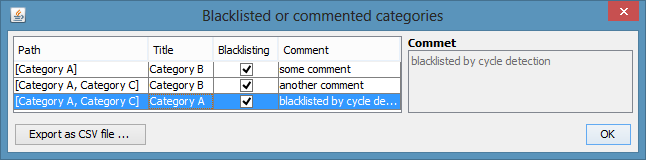
\includegraphics[scale=0.8]{figures/table_dialog.png}
\caption{The table dialog}
\label{fig:table_dialog}
\end{figure}

When clicking the \texttt{OK} button, the table dialog is closed and all changes are applied to the underlying tree view.

\subsection{Saving, loading and exporting results}
\label{sec:save}
The \texttt{File} menu contains three more functions: \texttt{Save}, \texttt{Load},  and \texttt{Export as JSON}. With \texttt{Save}, the underlying graph can be saved while with \texttt{Load}, a saved graph can be restored. As \emph{WikiTax} is based on JGraLab\footnote{\url{https://github.com/jgralab}, last visit 17th April 2013}, its dedicated TG format for serialising graphs is used to save and load (processed) category graphs. All relevant data for reconstructing the category tree - including the currently calculated statistics for each category node - are stored in the TG file. Furthermore, the category graph can be exported in form of a JSON file \cite{RFC4627} that consists of serialised vertices and edges.

\begin{lstlisting}[frame=single,captionpos=b,caption={Serialised graph in JSON format (shortened)},label={lst:json},language=json]
[
  {
    "id":1,
    "title":"Category A",
    ...
    "type":"Category"
  },
  {
    "start":1,
    "type":"Contains",
    "end":2
  },
  {
    "id":2,
    "title":"Page 1",
    "type":"Page"
  },
  {
    "start":1,
    ...
    "type":"HasSubcategory",
    "end":3
  },
  {
    "id":3,
    "title":"Category B",
    ...
    "type":"Category"
  }
  ...
]
\end{lstlisting}

Listing \ref{lst:json} shows a serialised JSON graph, which consists of five elements, forming a graph composed of three vertices and two edges. It describes a graph consisting of the category named \texttt{Category A} which is connected to the page named \texttt{Page 1} via a \texttt{Contains}-edge and which is also connected to the category named \texttt{Category B} via a \texttt{HasSubcategory}-edge. Every vertex has an \texttt{id} that the edges use to indicate their \texttt{start} and \texttt{end}. Moreover, each vertex is either a \texttt{Category} or a \texttt{Page} and each edge is either a \texttt{ContainsPage}- or a \texttt{HasSubcategory}-edge. Every vertex can have a \texttt{title} that is its corresponding Wikipedia title. Some other attributes that were omitted in the listing can be obtained from figure \ref{fig:full_schema}.

\begin{figure}[ht]
\centering
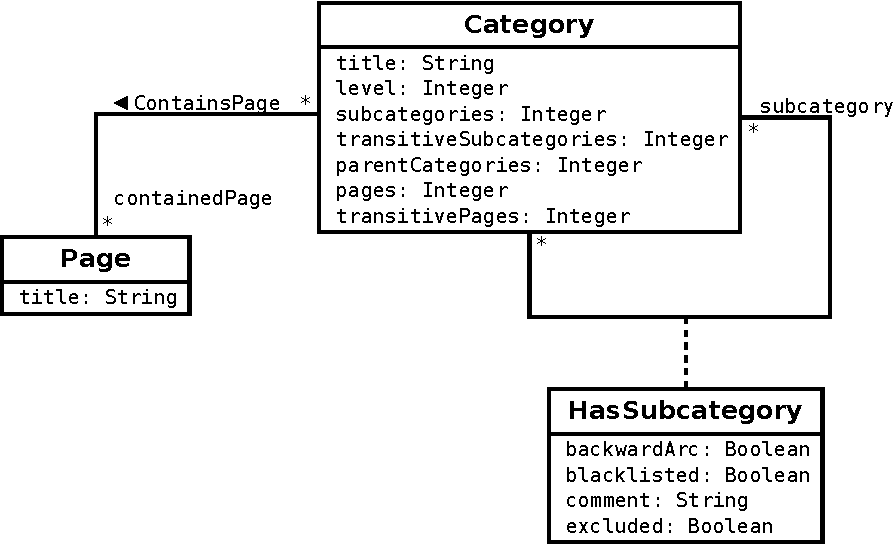
\includegraphics[width=0.63\textwidth]{figures/full_schema.pdf} 
\caption{Schema of the \emph{WikiTax} category graph}
\label{fig:full_schema}
\end{figure}

\section{Conclusion}
\label{sec:conclusion}
The developed tool \emph{WikiTax} provides basic functions to extract parts of the Wikipedia category graph and to reduce it iteratively in order to carve out the essential structure of Wikipedia. The concepts that are required for this process are explained in an application-oriented manner.

\emph{WikiTax} should be regarded as a prototypical implementation with the aim to visualise, analyse and extract relevant parts of the Wikipedia category graph. It was therefore generically designed and tested. Hence, it is essential to apply \emph{WikiTax} with a specific target in mind, rather than to perform generic tests while developing it. A need for adjustments of the highlighting modes or of the provided statistics could thus arise to improve the usability and suitability of the tool.

\bibliographystyle{alpha}
\bibliography{sources}

\end{document}
